\begin{quote}
	\textit{``The sinister thing about a simstim construct, really, was that it carried the suggestion that any environment might be unreal, that the windows of the shopfronts she passed now with Andrea might be figments.''}
\end{quote}
\hfill \textit{Count Zero, William Gibson}
\\
\\
\\

%=========================================================================================================
%=========================================================================================================

This chapter presents the development of a preliminary PR system that combined a tablet computer, GPS, accelerometer \& magnetometer, with an OpenSim based virtual environment to allow exploration of the real world ruins of a 14th century cathedral with a virtual reconstruction of it as it stood in its prime. Cultural heritage is introduced as an ideal area for which PR systems can be applied to beneficial effect, while the accuracy of GPS tracking emerged as a constraint on this style of interaction.

%=========================================================================================================

\section{Virtual Heritage}

Alternate reality technologies have been used for over two decades~\cite{Roussou2002} to aid in the investigation, understanding \& dissemination of information pertaining to our past, in the fields of archaeology \& cultural heritage. Whilst archaeology studies human activity through the recovery of remains, heritage is also concerned with intangible attributes of society; tradition, art, narratives \& other cultural evidences~\cite{Roussou2002}. \textit{Virtual heritage} is the name given to the application of advanced imaging techniques, including alternate reality techniques, for the synthesis, conservation, reproduction, representation, reprocessing \& display of this cultural evidence~\cite{roussou:photorealism}.

%=========================================================================================================

\subsection{Alternate Realities in Virtual Heritage}

Brief background/mini literature review on previous AR/VR projects in the heritage sector.

%=========================================================================================================

\subsection{Virtual Heritage at the University of St Andrews}

Background into the content that the group has produced, how it produced it, how it uses it, talk about different ways of interacting with it (including John's Kinect stuff, school children using \& enjoying Rift).

Lots of pictures of virtual content \& of people experiencing this content via the different interaction methods.

%=========================================================================================================

\section{The Virtual Time Window}

Introduce basic concept of VTW.

Talk about how previous alternate reality projects in cultural heritage have either been on-site AR, or VR with temporal/spatial separation. VTW allows on-site VR with no temporal/spatial separation. Bring in separation between Madras \& the cathedral.

%=========================================================================================================

\subsection{The Virtual Time Window within PR}

How with VTW we have a small `window' into the virtual, which is then surrounded by the real. So unlike Mirrorshades which is about distributing attention by time (one environment, then the other), VTW is about distributing attention by gaze/place (different parts of a single view/combined environment).

%=========================================================================================================

\section{Designing the Virtual Time Window}

How to interface sensor data with Second Life client - either try to make use of existing interfaces, or modify the client. Two approaches for using existing interfaces were explored; using an Arduino as a USB joystick \& using an OpenSim RegionModule to control avatar position from GPS data. But instead the Second Life client was modified to get both orientation \& GPS data.

%=========================================================================================================

\subsection{Second Life/OpenSim}

Talk about history of Second Life/OpenSim in academia/research, including original cross reality research.

The 3D virtual environment component of the Pangolin system was implemented using the Second Life/OpenSimulator (SL/OpenSim) platform, which provides a 3D social-oriented multi-user non-competitive virtual environment which focuses on the community, creation and commerce~\cite{Sevan2008} aspects of many users interacting within a shared space through the abstraction of avatars, rather than the competitive natures of games and the solitary environments commonly afforded by simulation and visualization platforms.

The distributed client/server model of SL/OpenSim, wherein 3D content is stored on a grid of servers operated by a multitude of organizations and distributed to and navigated between by dispersed clients on demand when they enter a particular region rather than being pre-distributed as is the norm for games, simulations and visualizations, is analogous to the manner in which 2D social Web content is served from Web servers to client browsers and apps.

This style of content delivery is necessary when considering the dynamic and ephemeral nature of consumer-generated media which constitutes the majority of the current 2D social Web and will make up the majority of expanding 3D social Web content.

%=========================================================================================================

\section{Orientation Control}

To control the SL camera in the required fashion, sensor data is collected for the direction that the user is facing (in terms of magnetic compass bearing) and the vertical angle (pitch) at which they are holding the tablet. Magnetic compass bearing is sensed using a magnetometer and pitch by an accelerometer. Roll data is also captured by the accelerometer, however it was expected that users would keep the tablet in a roughly horizontal fashion when interacting with it, thus using these data to control the SL camera's roll was not deemed to be beneficial and was not implemented.

The 110W does not feature a magnetometer and its tilt sensor is rudimentary (only useful for differentiating between discrete cases of landscape and portrait orientation for screen rotation). Several alternative sensors were auditioned, including the MMA8452, ADXL335, HMC5883L and eventually the HMC6343 which was adopted for the experiments. The HMC6343 combines a 3-axis magnetometer, 3-axis accelerometer and algorithms to internally apply the accelerometer's readings to tilt compensate the magnetometer's readings; tilt compensation is necessary for an accurate compass bearing when the device is not held in a perfectly level orientation, such as when the user tilts it up or down to view content above or below their eye level.

Magnetic declination information was entered into the HMC6343 for the position of the cathedral and the date of our experiments. The HMC6343's hard-iron offset calculation feature was used each time the hardware configuration was altered. The sampling frequency of the HMC6343 was set to its highest value of 10Hz. Orientation was set to `upright front' to match the physical orientation of the IC in the experiments.

%=========================================================================================================

\subsection{Exploiting the Second Life client's joystick support}

Leveraging standard SL avatar/camera control interfaces was explored by programming the Arduino to mimic a standard USB HID joystick via the Lightweight USB Framework for AVRs (LUFA), sending messages that the viewer interpreted as coming from a joystick and allowing the use of the standard joystick options.

\begin{figure}[h]
\centering
  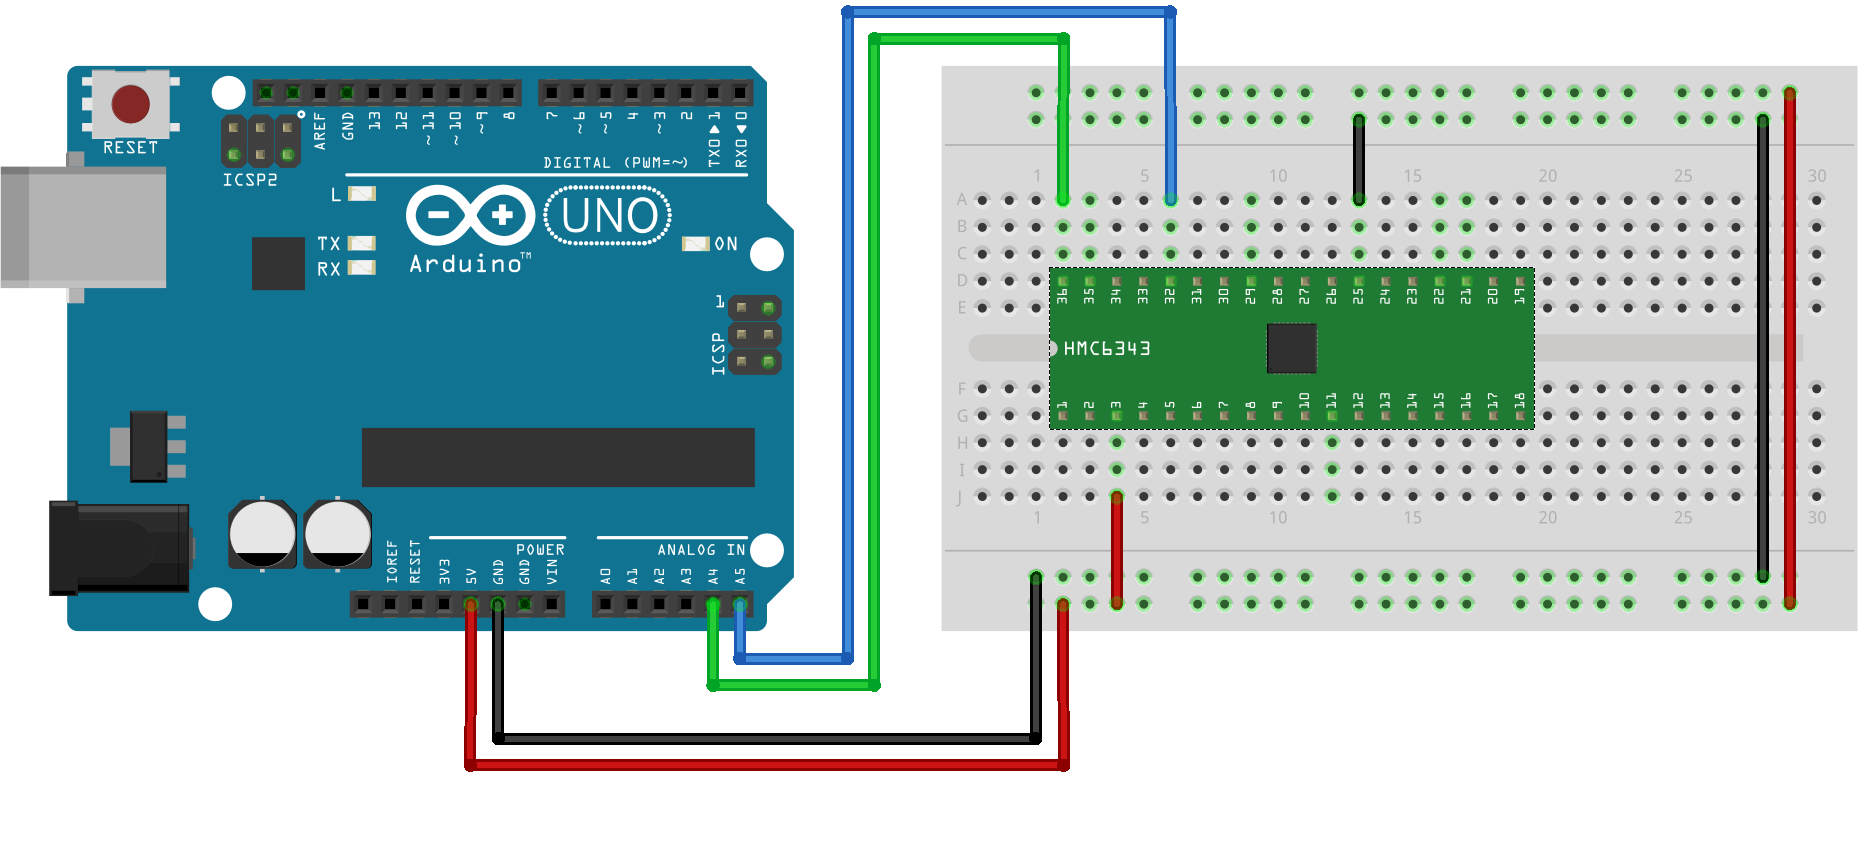
\includegraphics[width=\linewidth]{arduino_wiring_hmc.png}
  \caption{Example wiring for Arduino with HMC6343 for joystick operation.}
  \label{arduino_wiring_hmc.png}
\end{figure}

\begin{figure}[h]
\centering
  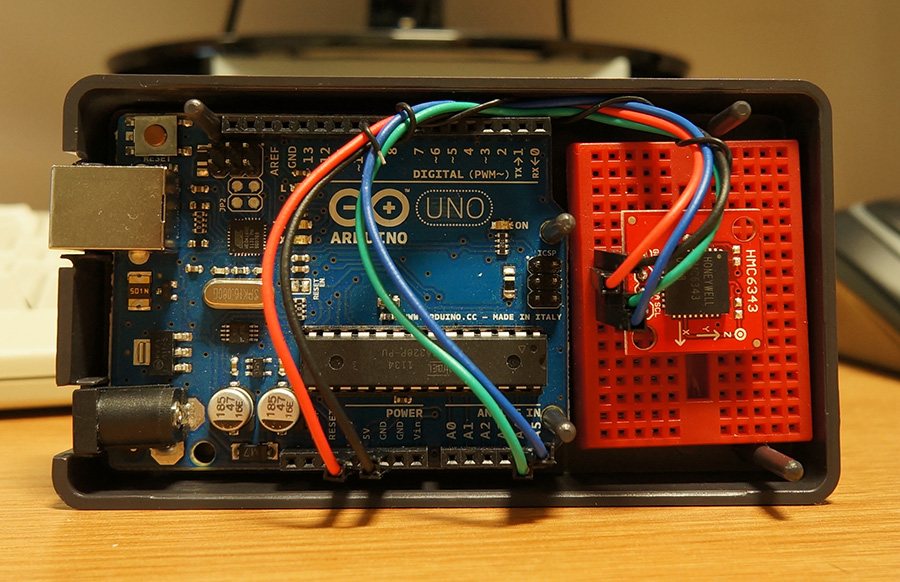
\includegraphics[width=.7\linewidth]{arduino_joystick_for_second_life_1.jpg}
  \caption{Assembled Arduino + HMC6343 `joystick'.}
  \label{arduino_joystick_for_second_life_1.jpg}
\end{figure}

\begin{figure}[h]
\centering
  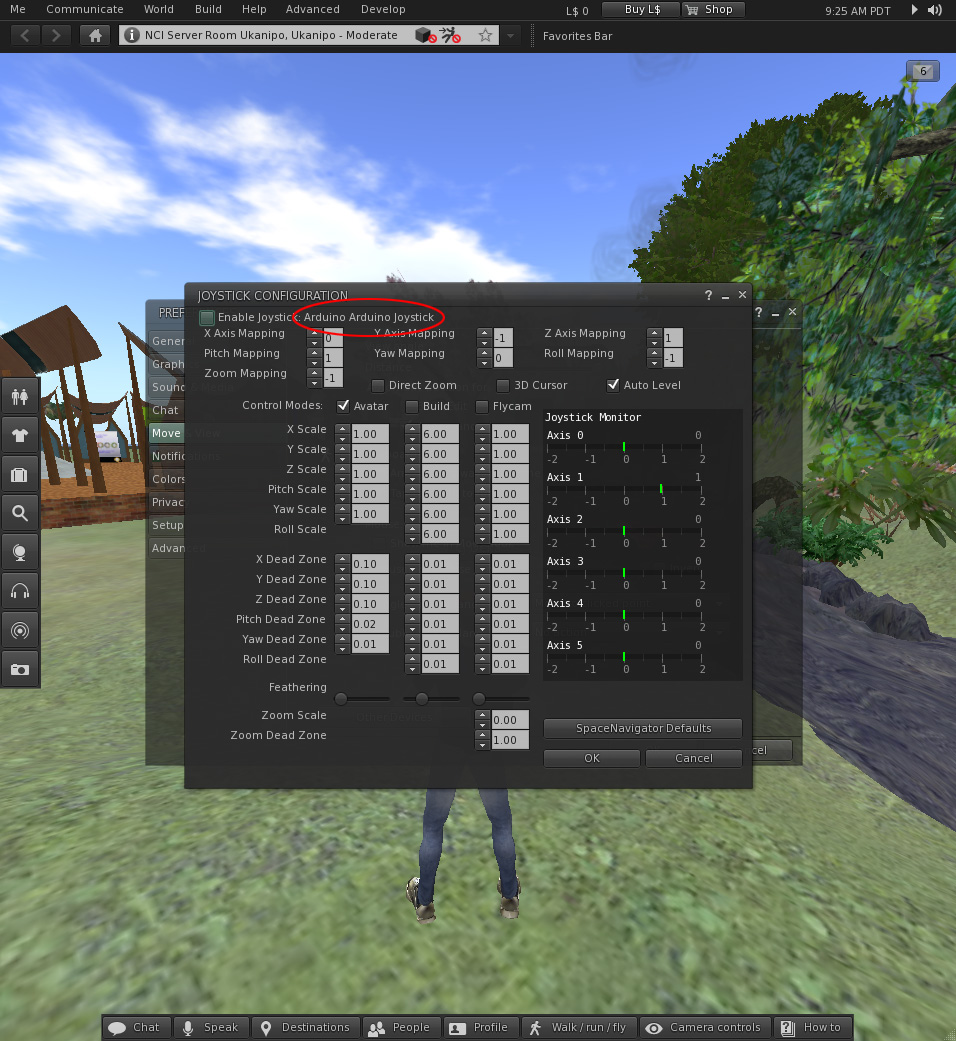
\includegraphics[width=\linewidth]{arduino_joystick_for_second_life_3.jpg}
  \caption{Configuration in Second Life client for Arduino + HMC6343 `joystick'.}
  \label{arduino_joystick_for_second_life_3.jpg}
\end{figure}

However the granularity of control attainable via this method was not sufficient.

%=========================================================================================================

\section{Position Control}

Translating real world positions, obtained via the GPS receiver as latitude and longitude pairs, into corresponding OpenSim (X,Y) region coordinates is achieved using the haversine formula~\cite{Gellert1989} from spherical trigonometry. The prerequisites for this approach are that the OpenSim model is aligned correctly to the OpenSim compass as the real location is aligned to real bearings (although provision to specify an `offset' within the Pangolin viewer for non-aligned models would be a trivial addition), that the model was created to a known and consistent scale and that a single `anchor point' is known for which both the real world latitude/longitude and corresponding OpenSim (X,Y) region coordinates are known.

Using the haversine formula the great-circle (or orthodromic) distance between the latitude of the anchor point and the latitude of the new GPS reading is calculated, then applying the scale of the model results in the equivalent distance in OpenSim metrics between the Y coordinate of the anchor point and the Y coordinate of the position corresponding to the new GPS reading. Repeating the same calculations with the longitude of the new GPS reading provides the distance between the X coordinate of the anchor point and the X coordinate of the position corresponding to the new GPS reading. Adding or subtracting these distances as appropriate to the OpenSim coordinates of the anchor point provides the OpenSim coordinates that correspond to the new GPS reading, to which the avatar is then instructed to move.

The anchor point is specified using global coordinates, not local coordinates. This allows navigation to operate across region boundaries and within mega regions (it is not limited to a single 256x256 meter OpenSim region) and there are no restrictions for the placement of the OpenSim component of the anchor point (it can be anywhere in any region, movement of the avatar can be in any direction from it (positive and negative), it does not have to be at the center of the model or even in a region that the model occupies).

Calculating a global coordinate is simply a case of multiplying the position of the region by 256 and then adding the local coordinate. For example, for an anchor at local coordinate $(127,203,23)$ within a region that is at $(1020,1042)$ the global X coordinate is calculated as $(1020 * 256) + 127 = 261247$ and the global Y coordinate as $(1043 * 256) + 203 = 267211$. Elevation (Z) is ignored due to a combination of the relatively low accuracy of these data attainable via GPS (when compared to the longitudinal/latitudinal accuracy) and as the case study explored involved users navigating outdoor ruins remaining at ground level.

%=========================================================================================================

\subsection{OpenSim RegionModule}

%=========================================================================================================

\section{Modifying the Second Life client}

%for both orientation \& position

The 110W features an AzureWave GPS-M16~\cite{AzureWave} GPS receiver; however poor API provision and meager documentation lead to use of a separate u-blox MAX-6 GPS receiver~\cite{U-bloxAG} outfitted with a Sarantel SL-1202 passive antenna~\cite{Sarantel}. The MAX-6 is of higher operational specification than the GPS-M16 and supports Satellite Based Augmentation Systems (SBAS) which improve the accuracy of location data by applying additional correction data received from networks of satellites and ground-based transmitters separate to those of the GPS system. These networks include the European Geostationary Navigation Overlay Service (EGNOS) that covers the UK where the experiments took place.

The product summary for the MAX-6 claims accuracy of 2.5m Circular Error Probable (CEP) without SBAS corrections and 2m CEP with SBAS corrections ``demonstrated with a good active antenna''~\cite{U-bloxAG2012}. This means that, in an ideal situation with SBAS correction data available, there would be 50\% certainty that each position reported by the GPS receiver would be within 2m of its actual position. The SL-1202 antenna used is passive, however as the distance between antenna and the MAX-6 IC itself in the hardware application is only a few millimeters there would have been negligible benefit from using an active antenna. However whether the SL-1202 constitutes `good' for achieving the headlining performance characteristics of the MAX-6 is debatable as the definition of `good' was not provided in the product summary.

The MAX-6 was operated in `pedestrian' dynamic platform model, use of SBAS correction data was enabled and frequency of readings was set to the maximum of 5Hz.

To determine the real world accuracy attainable with the MAX-6 outfitted with the SL-1202 in situations akin to those of the cultural heritage case study, a walking route around the St Andrews cathedral ruins, akin to the route that an individual visitor or school group might take, was planned and then walked with the MAX-6 connected to a laptop computer via an Arduino operating as a Universal Asynchronous Receiver/Transmitter (UART) feeding the raw National Marine Electronics Association (NMEA) messages into the `u-center'GPS evaluation software version 7.0 which logged the messages for later evaluation. Simultaneously for comparative purposes a mid-range consumer Android smartphone was used to record the same track; a HTC One S~\cite{HTCCorporation2013} containing a gpsOne Gen 8A solution within its Qualcomm Snapdragon S4 processor~\cite{QualcommIncorporated2013} and using Google's `My Tracks' app version 2.0.3 to record the data. The three sets of positional data (planned route, MAX-6 recorded route and smartphone recorded route) were entered into a PostgreSQL database~\cite{Daviesc,Daviesb} and the PostGIS database extender's ST\_HausdorffDistance algorithm~\cite{PostGIS} was used to calculate the Hausdorff distances between the recorded routes and the planned route and between the recorded routes themselves. In this scenario, the Hausdorff distance represents the furthest distance needed to travel from any point on the route recorded by the GPS receiver to reach the nearest point on the planned route. Because of the substantially greater inaccuracies identified in the latter part of the recorded tracks, separate Hausdorff distances were calculated both for the complete tracks and also for truncated first and second sub-tracks.

Whilst SL/OpenSim encapsulates many of the desirable architectural features for 3D PoSR experiments it does not support execution upon familiar mobile platforms (Android/iOS) nor does it provision for avatar control from sensor data. However the open source nature of the SL viewer allowed modifications to be effected, enabling control of the avatar and camera from real time data collected from position and orientation sensors connected to a tablet computer. This ability to control navigation within the 3D virtual environment without explicit conscious input of keyboard/mouse/touch commands is integral to reducing the cognitive load required to maintain a presence within a virtual environment which is a key requirement for overcoming the vacancy problem and achieving successful mobile cross reality.

As the SL viewer is only available for x86 platforms the choice of user hardware platform for the experiments was limited, with the MSI WindPad 110W presenting the most promising solution: a 10'' tablet computer sporting an AMD Brazos Z01 APU (combining a dual-core x86 CPU and Radeon HD6250 GPU)~\cite{Micro-StarInt'lCo.}. The user's position was monitored using GPS, a solution which is well suited to applications of the system within the use case of cultural heritage; such sites often constitute outdoor ruins at which a clear view of the sky allows for good GPS connectivity. For use cases where a similar modality of interaction is desired whilst indoors then an indoor positioning system would be used; a roundup of such technologies is available in~\cite{Mautz2012}.

To reduce computational load on the 110W, the OpenSim server was run on a separate Lenovo ThinkPad X61s laptop computer during the experiments. Due to the limited range of the laptop's wireless interface, the laptop was connected by RJ45 ethernet cable to a Linksys WRT54G wireless router to allow the 110W to access the OpenSim server wirelessly from anywhere within the experiment area. The router was powered from a 12V sealed lead-acid battery. This setup is shown in figure \ref{server}.



The TinyGPS library~\cite{Hart} was used to abstract processing of NMEA messages from the MAX-6 to obtain the required latitude and longitude values.

HMC6343 SDA A4
HMC6343 SCL A5

ublox TX digital 5
ublox RX digital 4

LED on digital 12

5v \& gnd where appropriate (boards used have step downs to 3.3v where required)

Go through Arduino sketch \& talk about things like magnetic declination, etc.

\begin{figure}[h]
\centering
  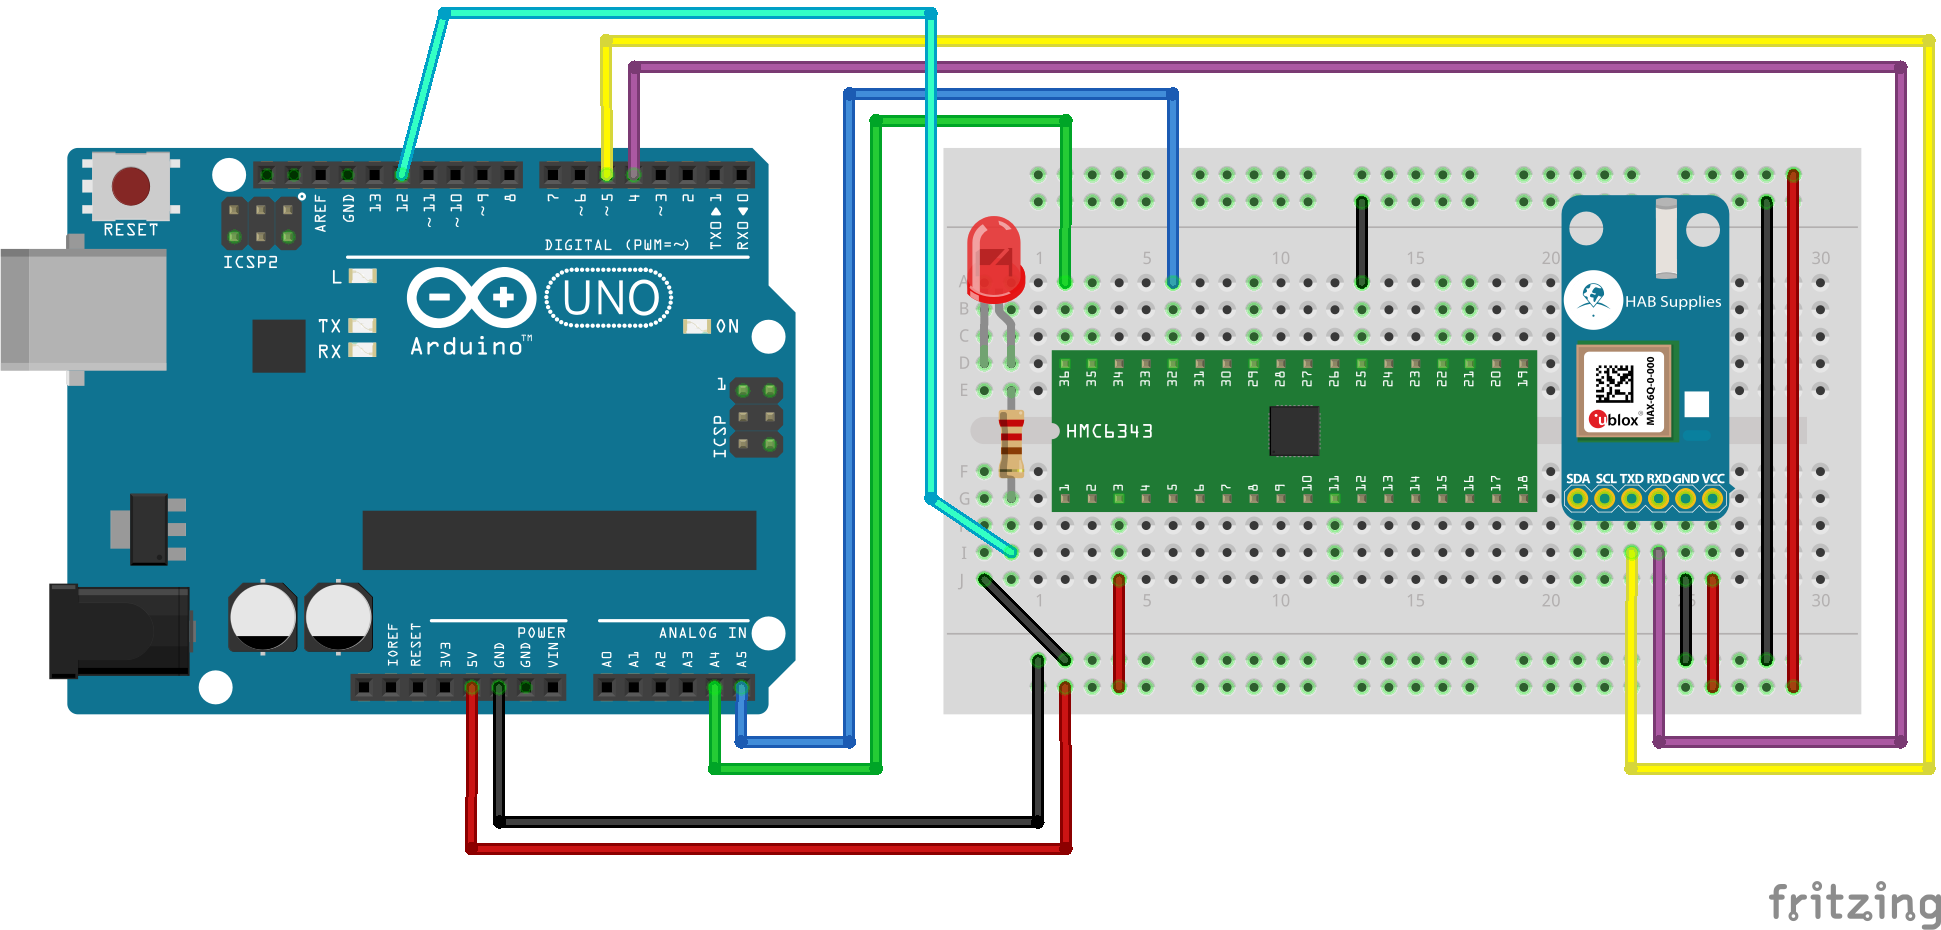
\includegraphics[width=\linewidth]{arduino_wiring_hmc_ublox.png}
  \caption{Example wiring for Arduino with HMC6343 + u-blox MAX-6.}
  \label{arduino_wiring_hmc_ublox.png}
\end{figure}

\begin{figure}[h]
\centering
\begin{minipage}{.5\textwidth}
 	\centering
 	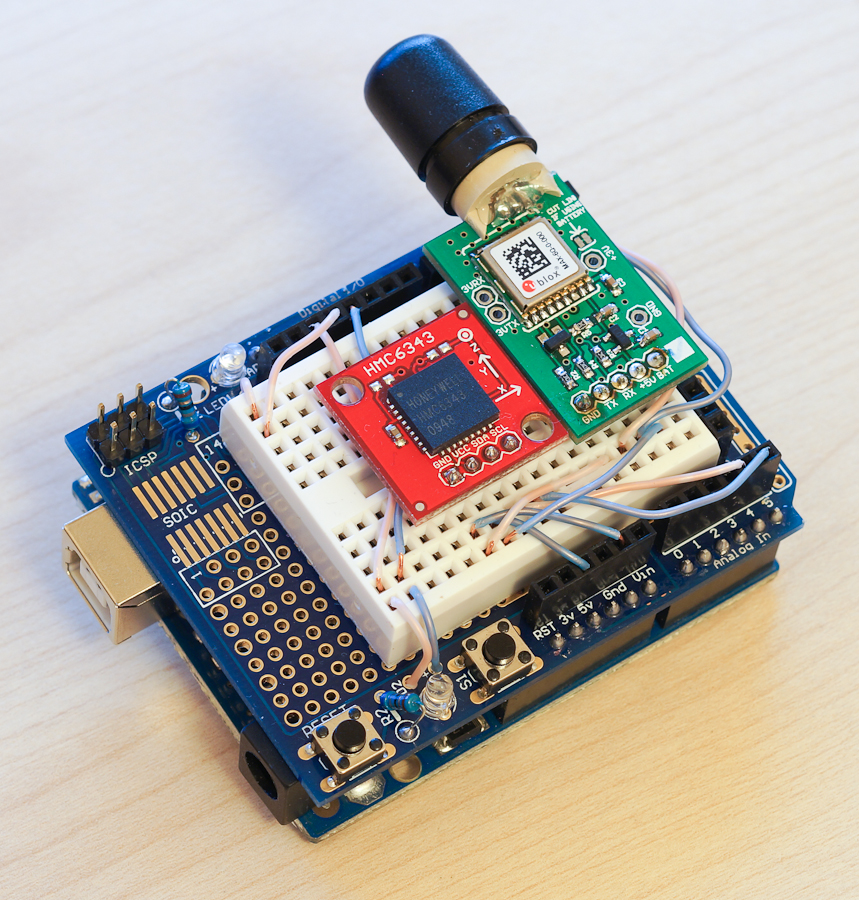
\includegraphics[width=0.95\linewidth]{arduino_hmc6343_u-blox_MAX-6.jpg}
 	\caption{Assembled Arduino + HMC6343 + u-blox MAX-6.}
	\label{arduino_hmc6343_u-blox_MAX-6.jpg}
\end{minipage}%
\begin{minipage}{.5\textwidth}
  \centering
  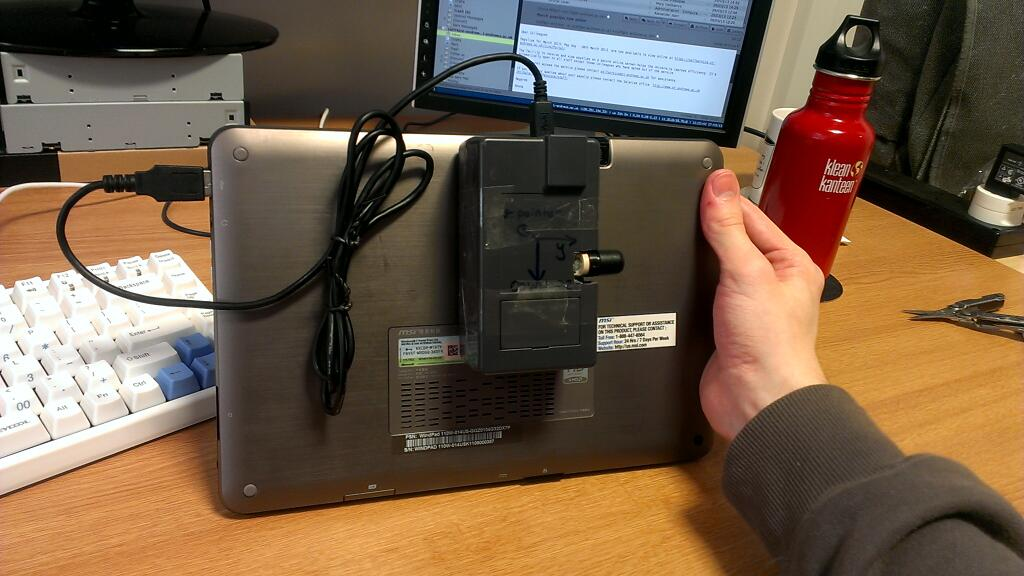
\includegraphics[width=0.95\linewidth]{pangolin_tablet_back.jpg}
    \caption{Arduino package attached to rear of tabet computer.}
    \label{pangolin_tablet_back.jpg}
\end{minipage}
\end{figure}

the viewer was modified (giving rise to the Pangolin viewer) to make use of the Boost.Asio C++ library to support receiving data via serial port and to use these data to control the movement of the avatar and camera by directly interfacing with the control functions at a lower level of abstraction. Receipt of messages is performed in an asynchronous non-blocking fashion, with the viewer's main loop processing the most recently received message in each iteration. Messages follow the format

$\langle bearing \rangle$ $\langle pitch \rangle$ $\langle roll \rangle$ $\langle latitude \rangle$ $\langle longitude \rangle$

The viewer's GUI was modified with the addition of a dialogue that allows the user to specify the path of the serial device, separately enable or disable sensor-driven camera and movement control, as well as providing numerous controls for fine-tuning its behavior, including the ability to specify high-pass filters for avatar movement and specify the smoothing applied to camera control. This GUI also presents the necessary fields for input of the anchor point details and fields for diagnostic output of the received information. Figure \ref{pangolin_screenshot} shows this GUI within the Pangolin viewer.

\begin{figure}[h]
\centering
  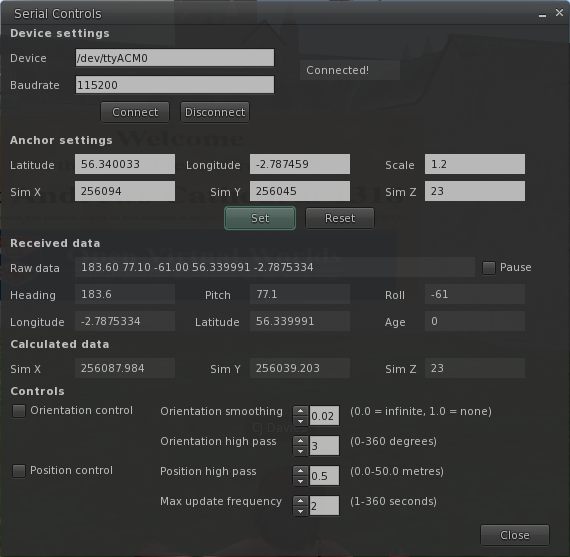
\includegraphics[width=0.7\linewidth]{pangolin_second_life_dialogue.png}
  \caption{Config pane in modified Second Life client for HMC6343 + MAX-6.}
  \label{pangolin_second_life_dialogue.png}
\end{figure}

%=========================================================================================================

\section{Using the Virtual Time Window}

\begin{figure}[h]
\centering
\begin{minipage}{.5\textwidth}
 	\centering
 	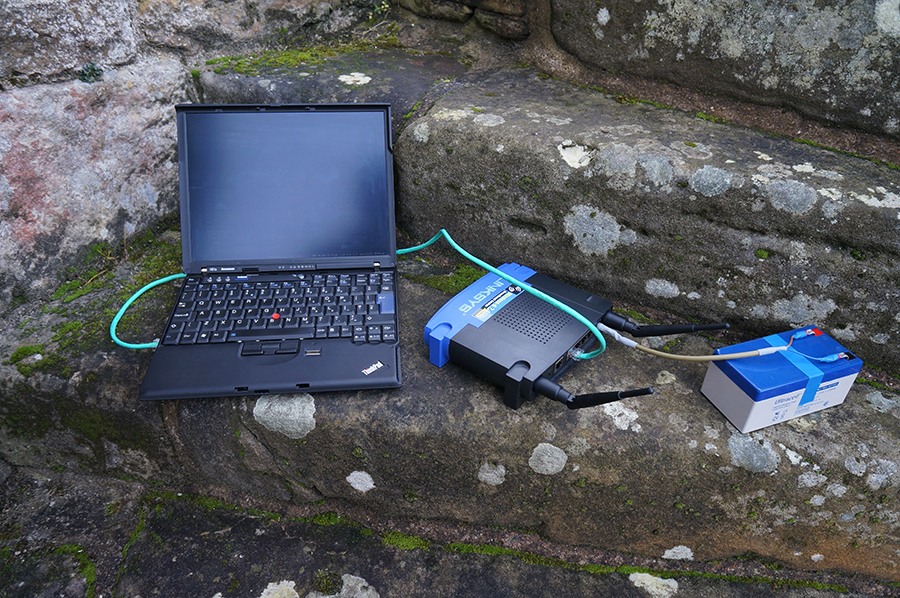
\includegraphics[width=0.95\linewidth]{pangolin_laptop_router_battery.jpg}
 	\caption{Server \& router provision for VTW use.}
	\label{pangolin_laptop_router_battery.jpg}
\end{minipage}%
\begin{minipage}{.5\textwidth}
  \centering
  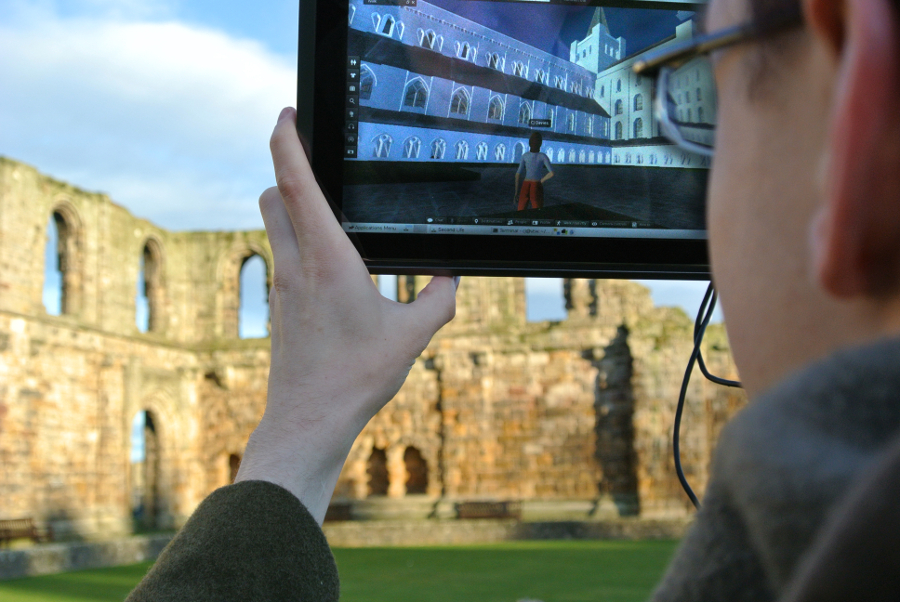
\includegraphics[width=0.95\linewidth]{pangolin_in_use.jpg}
    \caption{VTW in use at St Andrews cathedral.}
    \label{pangolin_in_use.jpg}
\end{minipage}
\end{figure}

Two plausible modalities of interaction were identified for this system, with each presenting different requirements with regards to accuracy of position tracking.

The first modality is one in which a number of locations that represent points of particular interest are identified. This is already a common practice at cultural heritage sites, with such locations often bearing signs or placards presenting text and/or images explaining what can be observed from the position. With Pangolin, when a user walks within a certain range of such a point, their avatar can be moved to the corresponding location within the reconstruction (and a sound played to alert the user to the fact that there is something of interest to observe) from which they can then move the tablet around them to examine their surroundings in the reconstruction. This modality is similar to audio tours employed by many museums and cultural heritage sites, but replaces the requirement to follow a static route or type in numbers of locations with the ability to freely navigate the real environment with access to additional information being triggered automatically once within the required range of a point of interest.

The second modality is one of free roaming exploration, in which the movements of the user's avatar within the reconstruction mimic the user's movements within the real world as closely as possible.
The first modality can be scaled to function with different accuracies of position tracking; as long as the distance between any two points of interest is at least as much as the worst case performance of the position tracking then distinguishing correctly between different points will always succeed. The second modality requires extremely accurate position tracking, arguably surpassing the capabilities of mainstream GPS technology even in ideal situations.

During the experiments the MAX-6 was unable to maintain reception of the additional correction data required for SBAS operation; when left stationary for several minutes reception was possible however subsequent movement of only a few meters at walking pace broke the connection. This reduced the theoretical maximum performance of the unit to 2.5m CEP, with observed performance being lower. Figure \ref{map_one} depicts an aerial view of the St Andrews cathedral ruins; the blue line represents the planned route, red the route recorded by the MAX-6 receiver and green the route recorded by the smartphone for comparative purposes, both while walking the planned route.

%\begin{figure}[h]
%\centering
%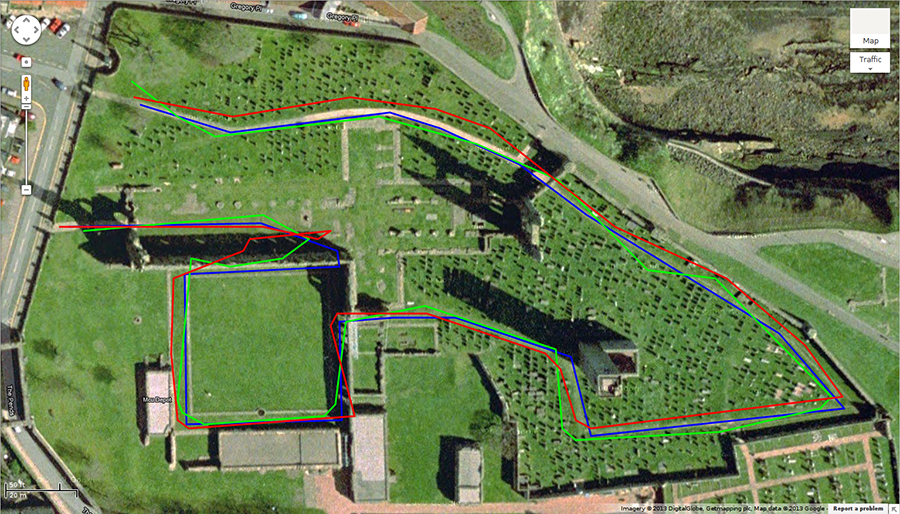
\includegraphics[width=0.48\textwidth]{images/figure_4}
%\caption{Aerial view oriented North upward of the St Andrews cathedral ruins; the blue line represents the planned route, red the route recorded by the MAX-6 and green the route recorded by the smartphone whilst walking the planned route.}
%\label{map_one}
%\end{figure}

The Hausdorff distance between the planned route and that recorded by the MAX-6 was $1.02e^{-04\circ}$. The `length' of a degree of latitude and a degree of longitude depends upon location upon the Earth; around the location of the St Andrews cathedral 1$^\circ$ of latitude is equivalent to 111347.95m and 1$^\circ$ of longitude to 61843.88m. Thus the Hausdorff distance of $1.02e^{-04\circ}$ can be visualized as $\pm11.3$m of North/South inaccuracy or $\pm6.3$m of East/West inaccuracy (or a combination of both N/S and E/W inaccuracy not exceeding a total displacement of $1.02e^{-04\circ}$ from the planned route).

The MAX-6 did achieve better performance than the smartphone, which recorded a Hausdorff distance of $1.33e^{-04\circ}$ ($\pm14.8$m N/S, $\pm8.2$m E/W). The Hausdorff distance between the routes logged by the MAX-6 and the smartphone was $1.14e^{-04\circ}$ ($\pm12.7$m N/S, $\pm7.0$m E/W), which represents a low correlation between the inaccuracies recorded by the two receivers even though they are of similar magnitudes from the planned route.

The maximum inaccuracies were recorded when walking along the South wall of the cathedral's nave. This wall is one of the most complete sections of the building with stonework reaching some 30ft above ground level and providing an effective obstruction to line-of-sight to half of the sky (and substantially impairing reception of signals from GPS satellites) when in close proximity to it. When considering just the sub-route shown in figure \ref{map_two}, which terminates before this wall begins to significantly obstruct view of the sky, the Hausdorff distances are notably smaller; the MAX-6 achieved a Hausdorff distance of $7.23e^{-05\circ}$ ($\pm8.05$m N/S, $\pm4.47$m E/W) throughout this sub-route, with the smartphone still behind with $8.99e^{-05\circ}$ ($\pm10.01$m N/S, $\pm5.56$m E/W). Again the Hausforff distance between the receivers showed low correlation between the inaccuracies, at $6.43e^{-05\circ}$ ($\pm7.12$m N/S, $\pm3.98$m E/W).
 
%\begin{figure}[h]
%\centering
%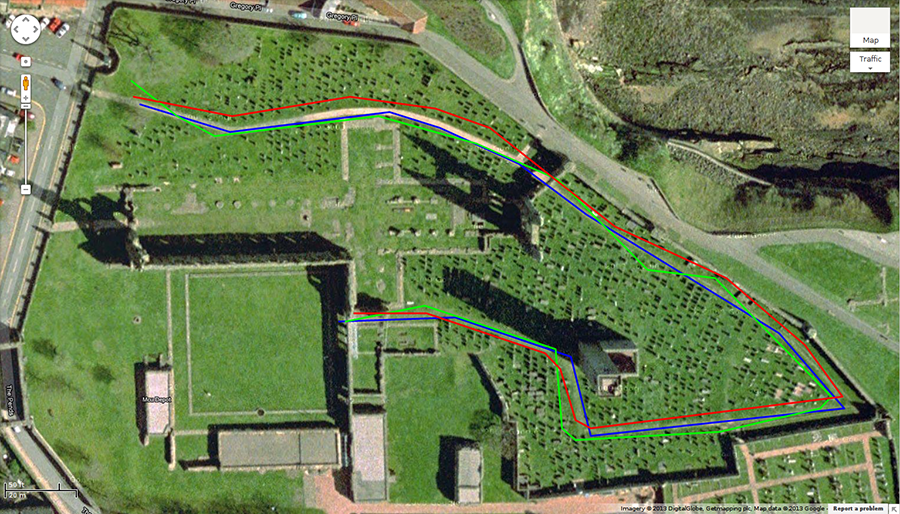
\includegraphics[width=0.48\textwidth]{images/figure_5}
%\caption{Aerial view oriented North upward of the St Andrews cathedral ruins; the blue line represents the first sub-route of the planned route, red the sub-route recorded by the MAX-6 and green the sub-route recorded by the smartphone whilst walking the first planned sub-route.}
%\label{map_two}
%\end{figure}

When analyzing the tracks in the vicinity of the nave (see figure \ref{map_three}) it is shown that although the MAX-6 outperformed the smartphone in terms of Hausdorff distance this relationship can be considered misleading as the smartphone track corresponded more closely in shape to the planned route even if it did stray further at its extreme. The discrepancy in the behavior of the two receivers in this situation is attributed to different implementations of dead-reckoning functionality between the receivers. Dead-reckoning is the process used when a GPS receiver loses reception of location data from satellites and extrapolates its position based upon a combination of the last received position data and the velocity of travel at the time of receiving these data.
 
%\begin{figure}[h]
%\centering
%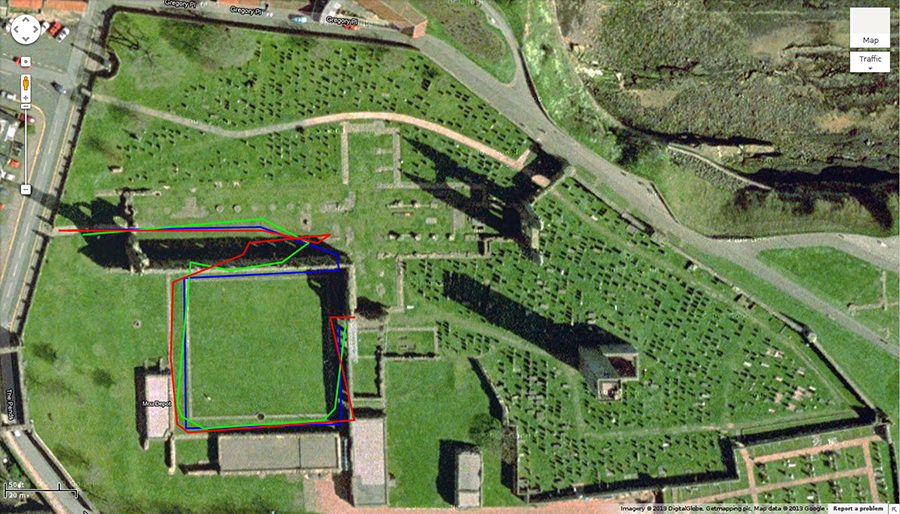
\includegraphics[width=0.48\textwidth]{images/figure_6}
%\caption{Aerial view oriented North upward of the St Andrews cathedral ruins; the blue line represents the second sub-route of the planned route, red the sub-route recorded by the MAX-6 and green the sub-route recorded by the smartphone whilst walking the second planned sub-route.}
%\label{map_three}
%\end{figure}

Pangolin's camera control from orientation data does not have as stringent performance criteria as the movement control from position data. Unlike augmented reality where sparse virtual content is superimposed upon a view of a real environment and the virtual objects must be placed accurately in order for the effect to work well, cross reality presents a complete virtual environment that is viewed `separately' or side-by-side with the real environment and thus discrepancies between orientation of real and virtual environments have a less detrimental effect to the experience. Although the accuracy of the camera control during the experiments was reported as being sufficient, the speed at which the camera orientation moved to match physical orientation was reported as being too slow, resulting in having to wait for the display to `catch up' to changes in orientation. This is attributed to the 10Hz sampling rate of the orientation sensors which, particularly after readings are combined for smoothing purposes to reduce jerky movement, resulted in too infrequent orientation updates. Frame rates within Pangolin whilst navigating the route averaged between 15 and 20 frames per second with the viewer's `quality and speed' slider set to the `low' position.

The style of explorative interaction with virtual content that this system employs is more resilient to input lag and low frame rates than other scenarios of interaction with virtual content such as fast paced competitive video games including First Person Shooters (FPS) [20], but overall user experience would nonetheless be improved by a faster sampling of orientation data and a higher frame rate. Additionally it should be noted that the cathedral reconstruction was created with relatively powerful desktop computers in mind as the primary deployment platform and has not been optimized for use on less powerful mobile platforms such as Pangolin. Performance of Pangolin on a less graphically complex OpenSim region (Salt Pan 2 [17]), that also depicts a reconstruction of a cultural heritage site, was better at 20 to 25 frames per second at the `low' position and between 15 and 20 frames per second at `high' (see figure 7).

%\begin{figure}[h]
%\centering
%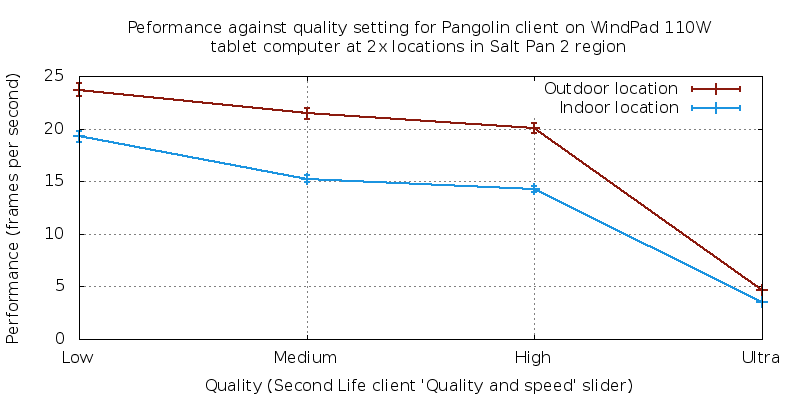
\includegraphics[width=0.48\textwidth]{images/figure_7}
%\caption{Plot of Pangolin's performance (measured in frames per second) against different graphical settings (selected via the `Quality and speed' slider of the viewer) in two positions within the Salt Pan 2 region.}
%\label{framerate_graph}
%\end{figure}

%\section{Interpretations}
The positional accuracy of $1.02e^{-04\circ}$ attained by the MAX-6 is sufficient for the first modality of interaction (that of distinguishing and navigating between multiple points of interest). This value of $1.02e^{-04\circ}$ (analogous to a combination of $\pm11.3$m of North/South inaccuracy or $\pm6.3$m of East/West inaccuracy) represents a constraint on the granularity of the content; it is the minimum distance required between any two points of interest for them to be correctly differentiated between. This same value is not sufficient for the second modality of interaction (that of free roaming exploration with avatars mimicking their users' movements as closely as possible). This modality would require the use of additional position tracking techniques to improve accuracy to around 1m CEP (analogous to $8.98e^{-06\circ}$ latitude or $1.62e^{-05\circ}$ longitude around the location of the St Andrews cathedral).

Use of a GPS receiver that is lower performance than the MAX-6 used by Pangolin, but more common due to being of the calibre integrated into smartphones and tablets such as that used in the experiments, is still sufficient for the first modality but with a larger minimum distance required between any two points of interest. The Hausdorff distance of $1.33e^{-04\circ}$ recorded by the smartphone used in the experiments is analogous to $\pm14.8$m N/S or $\pm8.2$m E/W around the location of the cathedral.

Observed accuracy of the orientation tracking is sufficient for both modalities of interaction; the accuracy of orientation tracking required does not change with different positional accuracy and the accuracy of orientation attained in the experiments is sufficient for an acceptable user experience, however the experience would benefit from better graphical quality and higher responsiveness to changes in user orientation.

%=========================================================================================================